\section*{Exercice 189 -- Modélisation}
\setcounter{exo}{0}
%CCS PSI 2009

\subsection*{Asservissement de position du palier magnétique actif}

Afin de satisfaire les critères du cahier des charges, on envisage d'asservir le
palier magnétique par un premier bouclage de stabilisation (retour $K_D p + K_P$).
Un second retour unitaire associé à un correcteur $C(p)$ assure la régulation en
position du palier.

\begin{center}
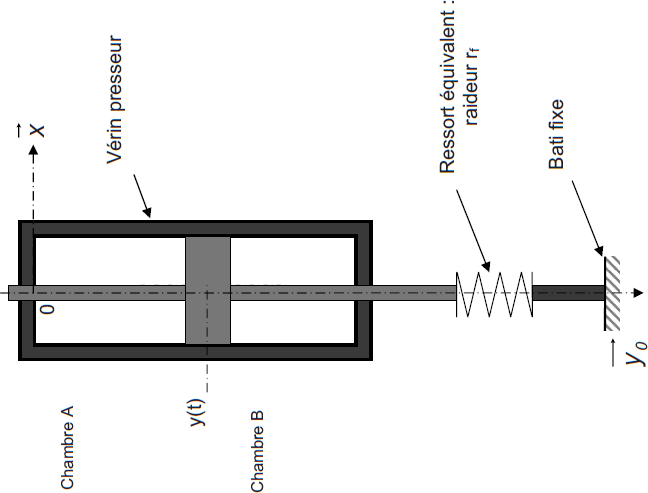
\includegraphics[width=\linewidth]{989_01}
\end{center}


On utilisera par la suite les paramètres suivants : $K_e = \SI{5000}{V.m^{-1}}$, $K_0 = \SI{190}{N.m^{-1}}$, $m=\SI{10}{kg}$.
On considère dans un premier temps le système sans correction : $C(p)=1$.


\subparagraph{}
 \textit{Déterminer la fonction de transfert de la boucle interne $H_{\text{PM I}}(p)=\dfrac{X(p)}{\varepsilon(p)}$, en fonction de $K_e$, $K_0$, $m$, $K_P$ et $K_D$. Préciser les conditions sur $K_P$ et $K_D$ pour que soit stable en boucle ouverte.}
\ifprof
\begin{corrige}
\end{corrige}
\else
\fi

\subparagraph{}
 \textit{En considérant l’ensemble de l’asservissement, déterminer la fonction de transfert 
 $H_{\text{pert}}(p)=\dfrac{X(p)}{F_{\text{pert}}(p)}$, puis calculer les valeurs de $K_D$ et $K_P$
permettant de respecter les spécifications du cahier des charges en terme de bande passante et d’amortissement.}
\ifprof
\begin{corrige}
\end{corrige}
\else
\fi


\begin{center}
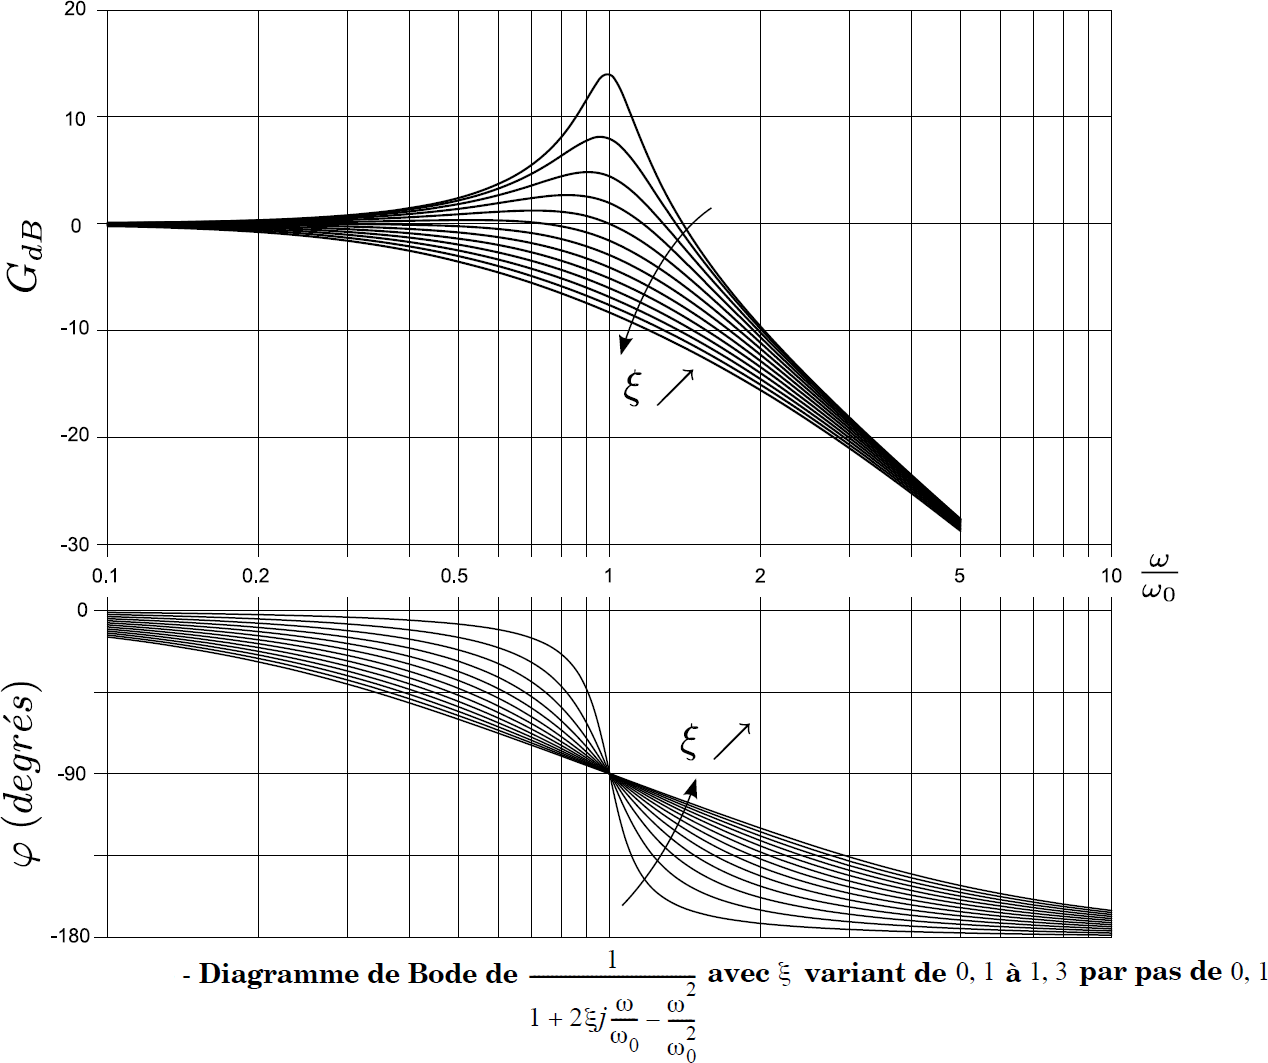
\includegraphics[width=\linewidth]{989_02}
\end{center}


\subparagraph{}
 \textit{}
\ifprof
\begin{corrige}
\end{corrige}
\else
\fi



\subparagraph{}
 \textit{Tracer l'allure des diagrammes de Bode asymptotique et réel de la fonction
de transfert de la boucle interne $H_{\text{PM I}}(p)$ et préciser la pulsation de coupure
ainsi que les marges de gain et de phase. Valider les critères de stabilité du
cahier des charges.}
\ifprof
\begin{corrige}
\end{corrige}
\else
\fi

L'ouverture et la fermeture des arrivées de gaz sont assurées par des « vannes
guillotines ». À la suite de la fermeture de la guillotine, le palier est soumis à un
effort bref mais violent, qui peut être modélisé par une perturbation d'effort en
échelon d'amplitude $F_G$.

\subparagraph{}
 \textit{Conclure quant au critère de sensibilité vis-à-vis des perturbations.}
 
 Afin d'améliorer les performances du système, on utilise un correcteur de fonction
de transfert $C(p)=K_i\left(1+\dfrac{1}{T_i p}\right)$.
 
\ifprof
\begin{corrige}
\end{corrige}
\else
\fi



\subparagraph{}
 \textit{}
\ifprof
\begin{corrige}
\end{corrige}
\else
\fi



\subparagraph{}
 \textit{}
\ifprof
\begin{corrige}
\end{corrige}
\else
\fi


\begin{enumerate}
\item ...
\item ...
\end{enumerate}